\documentclass[]{article}
\usepackage{lmodern}
\usepackage{amssymb,amsmath}
\usepackage{ifxetex,ifluatex}
\usepackage{fixltx2e} % provides \textsubscript
\ifnum 0\ifxetex 1\fi\ifluatex 1\fi=0 % if pdftex
  \usepackage[T1]{fontenc}
  \usepackage[utf8]{inputenc}
\else % if luatex or xelatex
  \ifxetex
    \usepackage{mathspec}
  \else
    \usepackage{fontspec}
  \fi
  \defaultfontfeatures{Ligatures=TeX,Scale=MatchLowercase}
\fi
% use upquote if available, for straight quotes in verbatim environments
\IfFileExists{upquote.sty}{\usepackage{upquote}}{}
% use microtype if available
\IfFileExists{microtype.sty}{%
\usepackage{microtype}
\UseMicrotypeSet[protrusion]{basicmath} % disable protrusion for tt fonts
}{}
\usepackage[margin=1in]{geometry}
\usepackage{hyperref}
\hypersetup{unicode=true,
            pdftitle={Direct Coefficient Recentering and Rescaling},
            pdfauthor={Doug Hemken},
            pdfborder={0 0 0},
            breaklinks=true}
\urlstyle{same}  % don't use monospace font for urls
\usepackage{graphicx,grffile}
\makeatletter
\def\maxwidth{\ifdim\Gin@nat@width>\linewidth\linewidth\else\Gin@nat@width\fi}
\def\maxheight{\ifdim\Gin@nat@height>\textheight\textheight\else\Gin@nat@height\fi}
\makeatother
% Scale images if necessary, so that they will not overflow the page
% margins by default, and it is still possible to overwrite the defaults
% using explicit options in \includegraphics[width, height, ...]{}
\setkeys{Gin}{width=\maxwidth,height=\maxheight,keepaspectratio}
\IfFileExists{parskip.sty}{%
\usepackage{parskip}
}{% else
\setlength{\parindent}{0pt}
\setlength{\parskip}{6pt plus 2pt minus 1pt}
}
\setlength{\emergencystretch}{3em}  % prevent overfull lines
\providecommand{\tightlist}{%
  \setlength{\itemsep}{0pt}\setlength{\parskip}{0pt}}
\setcounter{secnumdepth}{0}
% Redefines (sub)paragraphs to behave more like sections
\ifx\paragraph\undefined\else
\let\oldparagraph\paragraph
\renewcommand{\paragraph}[1]{\oldparagraph{#1}\mbox{}}
\fi
\ifx\subparagraph\undefined\else
\let\oldsubparagraph\subparagraph
\renewcommand{\subparagraph}[1]{\oldsubparagraph{#1}\mbox{}}
\fi

%%% Use protect on footnotes to avoid problems with footnotes in titles
\let\rmarkdownfootnote\footnote%
\def\footnote{\protect\rmarkdownfootnote}

%%% Change title format to be more compact
\usepackage{titling}

% Create subtitle command for use in maketitle
\newcommand{\subtitle}[1]{
  \posttitle{
    \begin{center}\large#1\end{center}
    }
}

\setlength{\droptitle}{-2em}

  \title{Direct Coefficient Recentering and Rescaling}
    \pretitle{\vspace{\droptitle}\centering\huge}
  \posttitle{\par}
    \author{Doug Hemken}
    \preauthor{\centering\large\emph}
  \postauthor{\par}
      \predate{\centering\large\emph}
  \postdate{\par}
    \date{2018-12-04}


\begin{document}
\maketitle

{
\setcounter{tocdepth}{1}
\tableofcontents
}

\hypertarget{introduction}{%
\section{Introduction}\label{introduction}}

For analysts working with linear models, recentering and rescaling the
variables under analysis is such a routine task it hardly garners
attention. In fields where there are no natural, physical units of
measurement - education and psychology, to name two - it is common
practice to refer to standardized units of measure. It is not uncommon
to see analysts fit and report the same model in both the original and
standardized units of measurement.

This is a classic problem, with a classic solution widely implemented in
statistical software, with well recognized limitations.

\hypertarget{the-problem-higher-order-models}{%
\section{The Problem: Higher Order
Models}\label{the-problem-higher-order-models}}

For additive models - models with intercepts and slopes of single
variables to polynomial degree one - the analyst can directly transform
the coefficients in the model via a classic formula that appears in most
textbooks. Consider, for example, the regression model
\[y = \beta_0 + \beta_1x_1 + \beta_2x_2\] where \(x_1\), \(x_2\), and
\(y\) are all continuous variables. If we transform the data so that all
the variables are centered, the transformed coefficients for this model
are given by \(\beta_0^\delta=0\) and \(\beta_i^\delta=\beta_i\) for
\(i\ge 1\). If we further transform the data so that all variables are
standardized, the transformed coefficients for this model are given by
\(\beta_0^z=0\) and \[\beta_i^z=\frac{\sigma_{x_i}}{\sigma_y}\beta_i\]

However, once interaction terms and higher order polynomial terms appear
in a model, using the classic formula requires recentering and rescaling
higher order terms with the means and standard deviations of the higher
order data vectors, the (Hadamard, element-wise) product of the lower
order data vectors, independent of the rescaling of lower order terms.

Consider, for example, the regression model
\[y = \beta_0 + \beta_1x_1 + \beta_2x_2+ \beta_3x_1x_2\] The classic
formula transforms \(\beta_0\), \(\beta_1\), and \(\beta_2\) as before.
For \(\beta_3\) we use the standard deviation of the product term
\(\sigma_{x_1x_2} (\neq \sigma_{x_1}\sigma_{x_2})\) as the numerator
rescaling factor. This implies that \(x_1x_2\) would have been
recentered with \(\mu_{x_1x_2}(\neq \mu_{x_1}\mu_{x_2})\), although we
do not need to actually calculate this. These are \textbf{\emph{not}}
the coefficients we would get if the data were first transformed, and
the model re-estimated.

This produces coefficients that are difficult to interpret because terms
involving the very same variables are on different scales. While this
can be useful for some purposes, such as calculating predicted values,
residuals, and goodness of fit, standard practice where the coefficients
are to be interpreted is to recalculate the data, then refit the model.
Refitting the model to recalculated data has the advantage that software
also produces a variance-covariance matrix appropriate to the
transformed coefficients, and sets up the software for post-estimation
operations with the transformed model.

Available software (SAS, Stata, SPSS) calculates standardized
coefficients directly using the classic approach, perhaps as a legacy of
the sweep operations of the 1970s. R has at least 3 packages -
QuantPsyc, lm.beta, and lsr - that implement this classic formula.

It seems to be little appreciated that the coefficients for recentered
and rescaled (including standardized) models can be easily calculated
directly.

\hypertarget{direct-transformation}{%
\section{Direct Transformation}\label{direct-transformation}}

\hypertarget{one-variable}{%
\subsection{One Variable}\label{one-variable}}

Transforming the coefficients and the variance-covariance matrix of a
linear model with a single continous outcome and a single continuous
predictor is straighforward. Consider the simple model
\[y = b_0 + b_1x\] or in the usual matrix form \[Y=X\beta\]

If we wish to recenter our model in terms of \(x_\delta=x-\mu_x\), an
arbitrarily recentered \(x\), we can do so without calculating the
\(x_\delta\). We use a linear transformation \(C\) to map the vector of
coefficients \(\beta\) to a vector of centered coefficients,
\(\beta^\delta\). \[\beta^\delta=C\beta\] where \(C\) takes the form
\[C=\begin{bmatrix}1 & \mu \\ 0 & 1 \end{bmatrix}\] Rescaling in terms
of \(x_z=x_\delta/\sigma\) can be done directly with the linear
transformation \[S=\begin{bmatrix}1 & 0 \\ 0 & \sigma \end{bmatrix}\] To
standardize the coefficients, we recenter, then rescale. In one step
this is
\[Z = S \times C =\begin{bmatrix}1 & \mu \\ 0 & \sigma \end{bmatrix}\]
To fully standardize this model, the final step is to standardize \(y\),
\(y_z=(y-\mu_y)/\sigma_y\). This requires adjusting \(\beta_0^z\) by
\(\mu_y\), which in this simple case leaves \(\beta_0^z=0\), and
dividing \(\beta^z/\sigma_y\). More complicated models also require
these two final operations for full standardization. It will simplify
further discussion to drop consideration of this.

It is worth noting that ``recentering'' and ``rescaling'' may be done
with any arbitrary constants, although it is perhaps most often done
with a sample mean and sample standard deviation. However, this same
approach would hold for converting a model where \(x\) is expressed, for
example, in degrees Fahrenheit to one expressed in degrees Centrigrade.

\hypertarget{example-one-variable-recentering}{%
\subsubsection{Example: One Variable
Recentering}\label{example-one-variable-recentering}}

\begin{verbatim}
example <- lm(mpg ~ wt, data=mtcars)
\end{verbatim}

Here the coefficients can be recentered as if the \(x\) variable
\texttt{wt} were recentered to the sample mean.

\begin{verbatim}
C <- matrix(c(1,0,mean(mtcars$wt),1), ncol=2)
C%*%coef(example)
\end{verbatim}

\begin{verbatim}
      [,1]
[1,] 20.09
[2,] -5.34
\end{verbatim}

We can check that this agrees with recentering the data, then refitting
the model.

\begin{verbatim}
wtcentered <- mtcars$wt - mean(mtcars$wt)
check <- lm(mpg ~ wtcentered, data=mtcars)
cbind(C%*%coef(example),coef(check))
\end{verbatim}

\begin{verbatim}
             [,1]  [,2]
(Intercept) 20.09 20.09
wtcentered  -5.34 -5.34
\end{verbatim}

We can also use the same recentering matrix to transform the
variance-covariance matrix of the coefficients.

\begin{verbatim}
C%*%vcov(example)%*%t(C)
\end{verbatim}

\begin{verbatim}
     [,1]  [,2]
[1,] 0.29 0.000
[2,] 0.00 0.313
\end{verbatim}

\begin{verbatim}
vcov(check)
\end{verbatim}

\begin{verbatim}
            (Intercept) wtcentered
(Intercept)        0.29      0.000
wtcentered         0.00      0.313
\end{verbatim}

\begin{verbatim}
# check equality
norm(C%*%vcov(example)%*%t(C)-vcov(check), "F")
\end{verbatim}

\begin{verbatim}
[1] 4.48e-16
\end{verbatim}

A change of basis for the column space of \(X\) induces a change of
basis for the column space of the coefficient vector, and a change of
basis for the row and column space of the variance-covariance matrix.
\(C\), \(S\), and \(Z\) are change of basis transformations.

\hypertarget{two-variables}{%
\subsection{Two Variables}\label{two-variables}}

Now consider a model with two continuous independent variables and an
interaction term, so the columns of \(X\) are
\(\begin{bmatrix} 1_n &x_1 &x_2 &x_1x_2 \end{bmatrix}\). We compose the
coefficient change of basis from the two simple transformations as a
direct product. Denote
\[C_1=\begin{bmatrix}1 & \mu_1 \\ 0 & 1 \end{bmatrix}\]
\[C_2=\begin{bmatrix}1 & \mu_2 \\ 0 & 1 \end{bmatrix}\] Then
\[C = C_2 \otimes C_1 = \begin{bmatrix} 1 & \mu_1 &\mu_2 &\mu_2\mu_1 \\
  0 &1 &0 &\mu_2 \\ 0 &0 &1 &\mu_1 \\ 0 &0 &0 &1 \end{bmatrix}\] The
classic standardization formula, as noted above, assumes recentering
with different constants in adjusting the coefficients. Note here that
recentering will always leave the highest order term unchanged.

While this transformation is simple to construct in theory, in practice
attention must be given to the column ordering: to use \(C\) we must
recognize that the column space is ordered
\(\begin{bmatrix} 1_n &x_1 &x_2 &x_1x_2 \end{bmatrix}\), so the order
must match that of the coefficient vector and the variance-covariance
matrix, perhaps through permutation.

While in general \(C_1 \otimes C_2 \neq C_2 \otimes C_1\), for any such
operation there exists a permutation, \(P\), such that
\(C_1 \otimes C_2 = P^T(C_2 \otimes C_1)P\). As long as we include
simple recentering and rescaling matrices for every variable used in our
coefficient terms, up to a final permutation their order does not
matter.

\hypertarget{example-two-variable-recentering}{%
\subsubsection{Example: Two Variable
Recentering}\label{example-two-variable-recentering}}

In order to build a recentering matrix, then, we need to collect a
labelled vector of recentering constants, and an ordered vector of
coefficient terms.

\begin{verbatim}
source("stdParm functions.r")

ex2 <- lm(mpg ~ wt*disp, data=mtcars)        # the base model
x.means <- colMeans(mtcars[,c("wt","disp")]) # recentering constants (means)
b.terms <- names(coef(ex2))                  # coefficients/terms

C <- recentering.matrix(x.means, b.terms)
C
\end{verbatim}

\begin{verbatim}
            (Intercept)   wt disp wt:disp
(Intercept)           1 3.22  231  742.29
wt                    0 1.00    0  230.72
disp                  0 0.00    1    3.22
wt:disp               0 0.00    0    1.00
\end{verbatim}

This, then, is what we use to produce recentered coefficients, and the
accompanying variance-covariance matrix.

\begin{verbatim}
C %*% coef(ex2)
\end{verbatim}

\begin{verbatim}
               [,1]
(Intercept) 18.8695
wt          -3.7950
disp        -0.0187
wt:disp      0.0117
\end{verbatim}

\begin{verbatim}
C %*% vcov(ex2) %*% C
\end{verbatim}

\begin{verbatim}
            (Intercept)      wt    disp  wt:disp
(Intercept)    -0.67299 -1.8682 -155.27  -431.03
wt             -1.84937 -4.8817 -426.70 -1126.34
disp            0.00716  0.0165    1.65     3.82
wt:disp         0.00826  0.0237    1.90     5.47
\end{verbatim}

\hypertarget{example-two-variable-rescaling}{%
\subsection{Example: Two Variable
Rescaling}\label{example-two-variable-rescaling}}

Rescaling is just as easy. Here,
\[S_1=\begin{bmatrix}1 &0 \\ 0 &\sigma_1 \end{bmatrix}\]
\[S_2=\begin{bmatrix}1 &0 \\ 0 &\sigma_2 \end{bmatrix}\] Then
\[S = S_2 \otimes S_1 = \begin{bmatrix} 1 &0 &0 &0 \\
  0 &\sigma_1 &0 &0 \\ 0 &0 &\sigma_2 &0 \\ 0 &0 &0 &\sigma_2\sigma_1 \end{bmatrix}\]
While the classic standardization formula takes a similar diagonal form,
the rescaling constants for higher order terms (\(>1\)) are different.

Rescaling can be useful independent of recentering, for example, to
rescale from United States customary units to SI units where the zero of
each scale remains unchanged.

\begin{verbatim}
# pounds to kilograms, and cubic inches to liters
x.scales <- c(1/453.592, 61.024)
names(x.scales) <- c("wt", "disp")
  
S <- recentering.matrix(x.scales, b.terms, type="scale")
S
\end{verbatim}

\begin{verbatim}
            (Intercept)     wt disp wt:disp
(Intercept)           1 0.0000    0   0.000
wt                    0 0.0022    0   0.000
disp                  0 0.0000   61   0.000
wt:disp               0 0.0000    0   0.135
\end{verbatim}

Check the coefficients:

\begin{verbatim}
wtkg  <- mtcars$wt*453.592  # 1000 lbs to kg
displ <- mtcars$disp/61.024 # cu.in. to liters

ex3 <- lm(mpg~wtkg*displ, data=mtcars)

ex3coefs <- cbind(S %*% coef(ex2),coef(ex3))
colnames(ex3coefs) <- c("Direct","Data Trans.")
ex3coefs
\end{verbatim}

\begin{verbatim}
              Direct Data Trans.
(Intercept) 44.08200    44.08200
wt          -0.01432    -0.01432
disp        -3.43920    -3.43920
wt:disp      0.00157     0.00157
\end{verbatim}

Compare the variance-covariance matrices:

\begin{verbatim}
norm(S %*% vcov(ex2) %*% S-vcov(ex3), "F")
\end{verbatim}

\begin{verbatim}
[1] 7.26e-15
\end{verbatim}

\hypertarget{interaction-terms-factorial-models-and-direct-products}{%
\section{Interaction Terms, Factorial Models, and Direct
Products}\label{interaction-terms-factorial-models-and-direct-products}}

To understand the use of the direct product here, we need to consider
the relationship between the \emph{data} space and the \emph{parameter}
space of a model. In all of the models considered here, the column space
of the parameters is a subset of the outer product of the columns space
of the data, including a column for the intercept term.

The data are modeled in an outer product of the data column space. In
transforming the coefficients, we need the same vector space for both
columns and rows - the Kronecker operator provides this twofold outer
product very neatly.

We may consider a model that includes only the mean of the response as a
zero-order model, sometimes called an intercept-only model. A model with
means of several categories, parameterized as a mean and offsets to that
mean, is a model with multiple intercepts (only), and is also a
zero-order model. Classical ANOVA models are zero-order models.

A model of a response with a continuous variable includes both an
intercept and a slope. This is a first-order model, with a zero-order
term and a first-order term. Adding categorical variables to the model
adds more intercepts, or zero-order terms. Adding continuous variables
adds more slopes, or first-order terms. Such additive models are all
first-order models.

An interaction term is formed as the product of two variables. A product
of categorical variables adds intercepts to the model. The interaction
of a categorical variable and a continuous variable adds slopes to the
model. In either case, the order of the model remains the same. But the
interaction formed from the product of two continuous variables adds a
second-order term to a model, a curvature.

A factorial model is formed by adding all the products of all the zero-
and first-order terms, in all combinations. If we think of the terms in
a model as its column space, then any linear model resides in a subspace
of the factorial column space. The columns of any linear model are a
subset of the columns in a full-factorial model.

Finally, transformations of the parameters are measured within the
parameter space. But transformations that reflect changes in the data
space are an outer product. Transformations from one basis for
parameters to another uses this outer product for both its column space
and row space. Kronecker operations give us just this result.

\hypertarget{less-than-full-factorial-models}{%
\section{Less-Than Full Factorial
Models}\label{less-than-full-factorial-models}}

A less-than-full factorial model can be though of as an outer product
with some terms zeroed out.

In practice, many models with interaction or polynomial terms are not
full factorial models. To derive the correct recentering and rescaling
matrices means realizing that some of the elements of \(\beta\) are
\(0\). Doing so allows us to work with reduced coefficient vectors and
reduced transformation matrices.

\hypertarget{dropping-higher-order-terms}{%
\subsection{Dropping Higher Order
Terms}\label{dropping-higher-order-terms}}

Consider again the additive model
\[y = \beta_0 + \beta_1x_1 + \beta_2x_2\]

The recentering matrix for \(x_1\) and \(x_2\) is as given above,
however for \(\beta\) we have
\[\begin{bmatrix}\beta_0^\delta \\ \beta_1^\delta \\ \beta_2^\delta \\ \beta_3^\delta \end{bmatrix}=
\begin{bmatrix} 1 & \mu_1 &\mu_2 &\mu_2\mu_1 \\
  0 &1 &0 &\mu_2 \\ 0 &0 &1 &\mu_1 \\ 0 &0 &0 &1 \end{bmatrix}
\begin{bmatrix}\beta_0 \\ \beta_1 \\ \beta_2 \\ 0 \end{bmatrix}\] This
simplifies to
\[\begin{bmatrix}\beta_0^\delta \\ \beta_1^\delta \\ \beta_2^\delta  \\ \beta_3^\delta \end{bmatrix}=
\begin{bmatrix} 1 & \mu_1 &\mu_2 \\
  0 &1 &0 \\ 0 &0 &1 \\ 0 &0 &0 \end{bmatrix}
\begin{bmatrix}\beta_0 \\ \beta_1 \\ \beta_2 \end{bmatrix}\] Not
surprisingly, this leaves \(\beta_3^\delta=0\), and we can further
simplify
\[\begin{bmatrix}\beta_0^\delta \\ \beta_1^\delta \\ \beta_2^\delta \end{bmatrix}=
\begin{bmatrix} 1 & \mu_1 &\mu_2 \\
  0 &1 &0 \\ 0 &0 &1 \end{bmatrix}
\begin{bmatrix}\beta_0 \\ \beta_1 \\ \beta_2 \end{bmatrix}\] In other
words, we end up with the only tranformation being to \(\beta_0\), which
had to be the result for a recentered additive model. Following this
approach for rescaling, we can derive in matrix form our classic
standardization formula for additive models as well.

\hypertarget{dropping-lower-order-terms}{%
\subsection{Dropping Lower Order
Terms}\label{dropping-lower-order-terms}}

Another point worth considering is the effect of recentering variables
on a model where a lower-order term has been dropped beneath a
higher-order term, such as a no-intercept model or a nested terms model.
Consider the model \[y = \beta_0 + \beta_1x_1 + \beta_3x_1x_2\] where
the term \(\beta_2x_2\) has been dropped, setting \(\beta_2=0\).

Here, our coefficient transformation looks like
\[\begin{bmatrix}\beta_0^\delta \\ \beta_1^\delta \\ \beta_2^\delta \\ \beta_3^\delta \end{bmatrix}=
\begin{bmatrix} 1 & \mu_1 &\mu_2 &\mu_2\mu_1 \\
  0 &1 &0 &\mu_2 \\ 0 &0 &1 &\mu_1 \\ 0 &0 &0 &1 \end{bmatrix}
\begin{bmatrix}\beta_0 \\ \beta_1 \\ 0 \\ \beta_3 \end{bmatrix}\] We can
simplify this somewhat as
\[\begin{bmatrix}\beta_0^\delta \\ \beta_1^\delta \\ \beta_2^\delta \\ \beta_3^\delta \end{bmatrix}=
\begin{bmatrix} 1 & \mu_1 &\mu_2\mu_1 \\
  0 &1 &\mu_2 \\ 0 &0 &\mu_1 \\ 0 &0 &1 \end{bmatrix}
\begin{bmatrix}\beta_0 \\ \beta_1 \\ \beta_3 \end{bmatrix}\] But here we
see that our recentered model gains a term and a coefficient,
\(\beta_2^\delta (=\mu_1\beta_3)\)!

The highest order term in which a variable appears is always unchanged
by recentering; lower order terms change when any of the \emph{other}
variables in a higher order term which includes the variables in the
lower order term are recentered. Going back to the additive model,
consisting of only first-order (slope) and zero-order (intercept) terms,
we see that only the intercept changes when the first order \(x_i\) are
recentered. Recentering a first-order model that had no intercept would
transform the coefficients so that an intercept was included.

If we build recentering and rescaling matrices variable by variable, we
can use less-than-full factorial combinations as building blocks. That
is to say, we could build a matrix for a full-factorial model and then
drop columns for unused terms, or we could approach this piecemeal.

{[}Checking for missing lower order terms in not currently implemented.
However, this should be easy to accomplish: drop columns in a full
factorial \(C\) or \(S\) not included in the coefficient vector
(i.e.~not among the terms), then check for rows that are zero vectors
and drop (only) those.{]}

\hypertarget{untransformed-variables}{%
\subsection{Untransformed Variables}\label{untransformed-variables}}

It may be that the analyst wishes to leave some variables untransformed.
One way to view this is that the recentering constant \(\mu=0\) and the
rescaling constant \(\sigma=1\). So the ``transformation'' for this
variable is just the identity matrix
\[S=C=\begin{bmatrix}1 & 0 \\ 0 &1 \end{bmatrix}\] This leads to a
simplification of the full factorial transformation matrix in terms of
direct sums. If we have \(C_2=I_2\), then
\[C_2 \otimes C_1 = \begin{bmatrix}C_1 &0 \\ 0 &C_1\end{bmatrix} = C_1 \oplus C_1 \]

\hypertarget{polynomial-terms}{%
\section{Polynomial Terms}\label{polynomial-terms}}

Polynomial models may also be built as outer products, but with lower
order terms collected.

Like less-than-full factorial models, models with polynomial terms are
worth a little extra scrutiny. Consider the model
\[y = \beta_0 + \beta_1x + \beta_3x^2\] If we rewrite this as
\[y = \beta_0 + \beta_1x + \beta_2x +\beta_3xx\] it looks like a
factorial model. But all the effect of \(x\) is collected in a single
term, \(\beta_1\), so \(\beta_2=0\). This is perhaps easier to see if we
look at the recentering transformation
\[\begin{bmatrix}\beta_0^\delta \\ \beta_1^\delta \\ \beta_2^\delta \\ \beta_3^\delta \end{bmatrix}=
\begin{bmatrix} 1 & \mu &\mu &\mu\mu \\
  0 &1 &0 &\mu \\ 0 &0 &1 &\mu \\ 0 &0 &0 &1 \end{bmatrix}
\begin{bmatrix}\beta_0 \\ \beta_1 \\ \beta_2 \\ \beta_3  \end{bmatrix}\]
If we take \(\beta_2=0\), then we can simplify as before
\[\begin{bmatrix}\beta_0^\delta \\ \beta_1^\delta \\ \beta_2^\delta \\ \beta_3^\delta \end{bmatrix}=
\begin{bmatrix} 1 & \mu &\mu\mu \\
  0 &1 &\mu \\ 0 &0 &\mu \\ 0 &0 &1 \end{bmatrix}
\begin{bmatrix}\beta_0 \\ \beta_1 \\ \beta_3  \end{bmatrix}\] But now
\(\beta_1^\delta\) and \(\beta_2^\delta\) both have part of the effect
of a recentered \(x_1\). If we collect these terms in
\(\beta^\delta_{12}=\beta_{1}^\delta+\beta_{2}^\delta\) we end up with
\[\begin{bmatrix}\beta_0^\delta \\ \beta_{12}^\delta \\ \beta_3^\delta \end{bmatrix}=
\begin{bmatrix} 1 & \mu &\mu\mu \\
  0 &1 &2\mu \\ 0 &0 &1 \end{bmatrix}
\begin{bmatrix}\beta_0 \\ \beta_1 \\ \beta_3  \end{bmatrix}\] Models
that include terms to any polynomial degree can be handled in this
manner.

Polynomial models where higher degree terms are included while dropping
lower degree terms, when recentered, will have the lower order terms
re-emerge, just as we saw with less-than-full factorial models with
dropped lower order terms.

Because rescaling transformation are diagonal matrices, the
simplification for a polynomial rescaling just drops a column and a row/

\hypertarget{categorical-terms}{%
\section{Categorical terms}\label{categorical-terms}}

In practice there are a number of approaches used for categorical
variables, i.e. collections of indicator/contrast variables.

\begin{itemize}
\tightlist
\item
  Leaving the intercept terms in reference coding amounts to leaving the
  coefficients for indicators untransformed, as described previously.
  Where there are \(k\) categories, then, we may use an \(I_k\) identity
  matrix, and do our computation are direct sums.
\item
  Standardizing each term as a z-score is equivalent to treating each
  category in the same manner as continuous variables, as described
  previously.
\item
  Transforming to coding other than reference coding is again a
  ``recentering'' change of basis in that it changes where we find zero
  in the parameter space. Here, however, we need another simple
  transformation.
\end{itemize}

For example, the general form of the reference coding to grand-mean
coding recentering matrix for a categorical variable with \(k\)
categories is \[
\begin{bmatrix}
1 &1/k     &\cdots &1/k \\
0 &(k-1)/k &\cdots &-1/k \\
0 &-1/k    &\cdots &-1/k \\
\vdots &\vdots &\vdots &\vdots \\
0 &-1/k    &\cdots &(k-1)/k
\end{bmatrix}
\]

This is then used in the same way as previously discussed recentering
transformations. (The first category remains the dropped column in this
transformation.)

\begin{verbatim}
C1 <- ref.to.gm(3)
rownames(C1) <- colnames(C1) <- c("(Intercept)", "cyl6", "cyl8")
C1
\end{verbatim}

\begin{verbatim}
            (Intercept)   cyl6   cyl8
(Intercept)           1  0.333  0.333
cyl6                  0  0.667 -0.333
cyl8                  0 -0.333  0.667
\end{verbatim}

Combined with our transformation matrix for a continuous variable

\begin{verbatim}
wtmean <- mean(mtcars$wt)
names(wtmean) <- "wt"
C2 <- mean.to.matrix(wtmean)
C <- kron(C2,C1)
C
\end{verbatim}

\begin{verbatim}
            (Intercept)   cyl6   cyl8   wt cyl6:wt cyl8:wt
(Intercept)           1  0.333  0.333 3.22   1.072   1.072
cyl6                  0  0.667 -0.333 0.00   2.145  -1.072
cyl8                  0 -0.333  0.667 0.00  -1.072   2.145
wt                    0  0.000  0.000 1.00   0.333   0.333
cyl6:wt               0  0.000  0.000 0.00   0.667  -0.333
cyl8:wt               0  0.000  0.000 0.00  -0.333   0.667
\end{verbatim}

This converts an uncentered model with reference coding for the
indicators to centered \texttt{wt} and grand-mean centered \texttt{cyl}.

\begin{verbatim}
cylf <- as.factor(mtcars$cyl)
excat <- lm(mpg ~ cylf*wt, data=mtcars)
summary(excat)
\end{verbatim}

\begin{verbatim}

Call:
lm(formula = mpg ~ cylf * wt, data = mtcars)

Residuals:
   Min     1Q Median     3Q    Max 
-4.151 -1.380 -0.639  1.494  5.252 

Coefficients:
            Estimate Std. Error t value Pr(>|t|)    
(Intercept)    39.57       3.19   12.39  2.1e-12 ***
cylf6         -11.16       9.36   -1.19  0.24358    
cylf8         -15.70       4.84   -3.24  0.00322 ** 
wt             -5.65       1.36   -4.15  0.00031 ***
cylf6:wt        2.87       3.12    0.92  0.36620    
cylf8:wt        3.45       1.63    2.12  0.04344 *  
---
Signif. codes:  0 '***' 0.001 '**' 0.01 '*' 0.05 '.' 0.1 ' ' 1

Residual standard error: 2.45 on 26 degrees of freedom
Multiple R-squared:  0.862, Adjusted R-squared:  0.835 
F-statistic: 32.4 on 5 and 26 DF,  p-value: 2.26e-10
\end{verbatim}

\begin{verbatim}
C %*% coef(excat)
\end{verbatim}

\begin{verbatim}
              [,1]
(Intercept) 19.227
cyl6         0.237
cyl8        -2.413
wt          -3.540
cyl6:wt      0.760
cyl8:wt      1.347
\end{verbatim}

\begin{verbatim}
contrasts(cylf) <- contr.sum
coef(lm(mpg~cylf*wtcentered, data=mtcars)) # note different dropped level
\end{verbatim}

\begin{verbatim}
     (Intercept)            cylf1            cylf2       wtcentered 
          19.227            2.176            0.237           -3.540 
cylf1:wtcentered cylf2:wtcentered 
          -2.107            0.760 
\end{verbatim}

\hypertarget{implementation}{%
\section{Implementation}\label{implementation}}

The basic algorithm here, the Kronecker product, is as old as the hills
and implemented in any software that handles matrix operations.
Integrating the pieces into useful software requires a little more work.

A useful implementation would take as input:

\begin{itemize}
\tightlist
\item
  a vector of recentering constants, labeled, one per variable in the
  model
\item
  a vector of rescaling constants, labeled, one per variable
\item
  a vector of coefficient terms (the labels themselves), formed so that
  constituent variables and polynomial degree can be extracted from each
  term
\end{itemize}

As implemented so far (the \texttt{recentering.matrix()} R function in
the two-variable examples above, (which calculates both recentering and
rescaling matrices) this handles less-than-full factorial models.
Missing from this implementation are:

\begin{itemize}
\tightlist
\item
  handling dropped lower order terms
\item
  handling polynomials
\item
  handling categorical contrast conversions
\end{itemize}

The algorithm for collecting like terms in a transformation matrix
(\texttt{collect.terms()}), for a single variable taken to an arbitrary
polynomial degree, is ready, but not yet integrated into the full
construction algorithm.

A useful computational simplification not yet fully implemented is:

\begin{itemize}
\tightlist
\item
  using direct sums for untransformed variables and collections of
  categorical indicators, rather than direct products,
  \texttt{factor.direct.sum()}.
\end{itemize}

Source code can be found at \url{https://github.com/Hemken/stdParm-R}

\hypertarget{errors-in-predictions}{%
\section{Errors in Predictions}\label{errors-in-predictions}}

The main benefit of direct transformation is improved interpretability,
and the general utility of the results for any post-estimation
calculation, without the cost of recalculating all the data values and
re-estimating the model.

An additional benefit is the reduction of numerical error.

In principle, the predicted values from the original model should be
exactly equal to the predicted values from a model estimated from the
centered data.

Here we compare two different methods of generating model coefficients
for recentered data. In the first method, we actually recenter the data,
then re-estimate the model, then calculate predicted values. In the
second method, we calculate the model coefficients directly, without
re-estimating the model. Then we calculate predicted values (using the
same recentered data as in the first method).

The model is
\[ y = \beta_0 + \beta_1x_1 +\beta_2x_2 + \beta_3x_3 + \beta_4x_1x_2 + 
\beta_5x_1x_3 + \beta_6x_2x_3 + \beta_7x_1x_2x_3\]

\hypertarget{simulation}{%
\subsection{Simulation}\label{simulation}}

\begin{itemize}
\tightlist
\item
  Numerical results: first is recentered data, second is directly
  recentered coefficients
\item
  Graphical results: black is recentered data, red is directly
  recentered coefficients
\end{itemize}

The numerical results are the mean norm of the difference between the
predicted values of the original model versus each of the coefficient
transformation methods - recalculation and direct transformation.

The graphical results are a kernel density plot of the normed
differences for each simulation.

All of the differences are tiny. The differences visible in the graph
are attributable to the QR estimation for the re-estimation method.

\begin{verbatim}
library(parallel)
cl <- makeCluster(8)

nvals <- 100L
clusterExport(cl, c("nvals", "sim.3var.center", "gen_3x", 
                    "mean.to.matrix", "matching.terms", "vars.in.terms", "kron",
                    "clean.kron.names", "matrix.build.clean"))
devnorms <- parSapply(cl, 1:100000, sim.3var.center, nvals)
rowMeans(devnorms)
\end{verbatim}

\begin{verbatim}
[1] 1.39e-14  6.70e-15
\end{verbatim}

\begin{verbatim}
kd.plot.overlay(t(devnorms), nvals)
\end{verbatim}

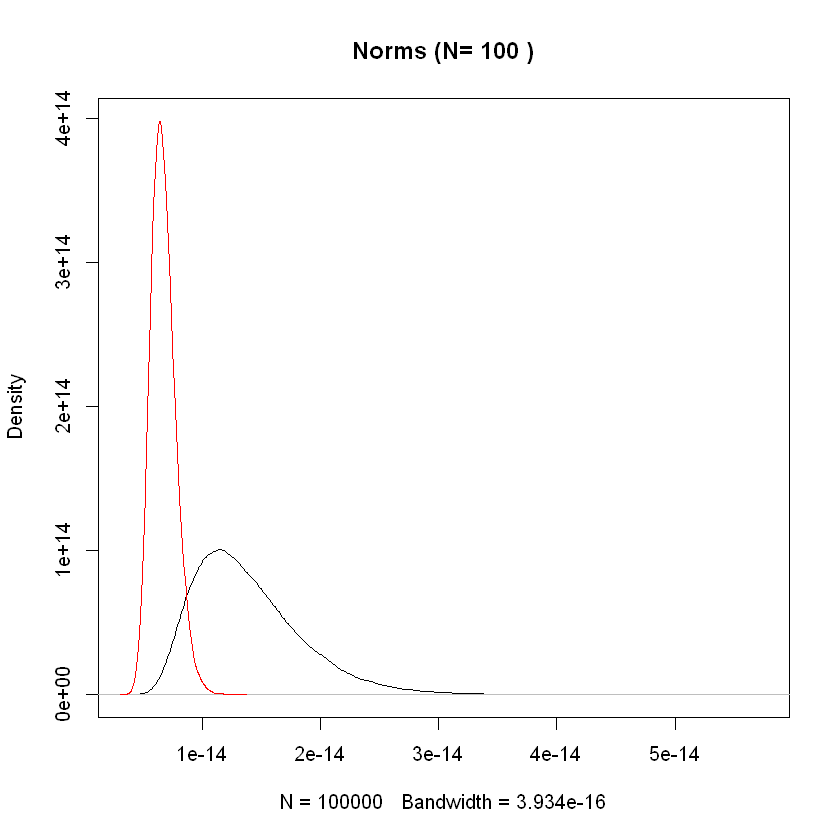
\includegraphics{errors/output_6_1.png}


\end{document}
